\documentclass{article}
\usepackage{longtable}
\usepackage{graphicx}
\usepackage{booktabs}% http://ctan.org/pkg/booktabs
\usepackage{xcolor}
\newcommand{\tabitem}{~~\llap{\textbullet}~~}
\newcommand\mytodo[1]{\textcolor{red}{#1}}
\usepackage{array}
\usepackage[style=numeric,backend=bibtex]{biblatex}
\usepackage{caption}
\usepackage{amsmath}

\bibliography{Parking}

\begin{document}

\title{SoNah Parking Analytics \\ \large (working title)}
\author{Andrei Ionita}

\maketitle

\section{Introduction}
\subsection{Conventions}
The following terms will be used throughout this document:
\begin{itemize}
\item \textbf{parking spot} - a single parking place
\item \textbf{parking location} - a space consisting of multiple parking places and is considered an unit
\end{itemize}

\section{Data Acquisition}
Data is certainly "the meat" of any Information System. It can broadly be split into two parts: direct parking- and contextual data. The former consist generally of parking snapshots, i.e. parking situations at a certain moment in time, e.g. 71 parking spots are now free, parking spot \#42 got occupied on Dec 12th. Contextual data refer to the geographical infrastructure where parking locations are represented, i.e. type of parking (free, for customers, for employees), "no parking" spots, relevant businesses in the area that lead to parking occupancy, etc.

\subsection{Parking-Data Snapshots}
\begin{enumerate}
\item \textbf{Sensor Data} --- the optical sensors deliver data records consisting of status change per parking spot; the format is: location (latitude, longitude), timestamp and parking spot status
\item \textbf{Parking Meter Data} --- consists of the number of tickets that have been purchased in a time period, e.g. day; this number alone does not offer direct information about the total number of parked vehicles during the certain time period, i.e. cars with permanent permission are not included, neither ticket dodgers
\item \textbf{Car Park Data} - the current number of free parking spaces in the city car parks as they are available online
\end{enumerate}

\subsection{Parking Geographical Information}
\begin{enumerate}
\item \textbf{Open Street Map} ---- OSM is an open Geographical Information System (GIS) platform where content is contributed by users. OSM is able to store detailed parking information consisting of location, type of parking (public, customers, company, etc.), parking fee, parking capacity, and others attributes.
\item \textbf{User-Generated Data} --- a smartphone application asks the users to introduce pieces of information about parking areas at their convenience, e.g. disabled parking spots, number of current free parking spots, type of business in the building nearby etc. Some of the information asked for is intentionally redundant, in order to cross-validate data from other sources. The users will hence have a stake at improving the parking-related infrastructure. 
\end{enumerate}

\subsection{Other contextual information}
\begin{enumerate}
\item \textbf{Events} --- whether concerts, sporting events, Christmas markets or others, events can greatly impact parking occupancy for certain periods of time. Therefore gaining access to the time and place of events makes sense
\item \textbf{Weather Conditions} --- dry, rainy or snowy weather plays a large role when deciding to use a car in the city and hence impacts parking as well
\item \textbf{Traffic Flow / Construction Sites} --- investigating the correlation between high/low traffic and nearby parking locations may help in improving parking prediction. That is why gaining access to traffic flow data and temporary construction site locations is important
\end{enumerate}

\subsection{Access to Data}
As soon as we discover a useful data source, gaining access to it is essential. Internal data will be saved in our \textbf{database}s. In case of Parking Snapshots, a NoSQL database will be used, since these are committed very frequently and non-relationality offers the advantage of easier processing, i.e. by using map/reduce, etc. Static data like geographical infrastructure shall conveniently be stored inside a relational database.

External data is at best accessed via an \textbf{Application Programming Interface (API)}, preferably REST, since this paradigm simplifies HTTP request/response processing; nevertheless, we accept querying other kinds of APIs too.

When external information is not explicitly made available, we investigate the approach of \textbf{crawling} or scraping the providers' web-sites. Scraping is the process in regular expressions are matched against retrieved HTML content in order to "clip out" interesting information. Before any external party content is retrieved however, we will make sure to comply with the law in this respect and will check whether the certain web-sites are crawlable at all.

\subsection{Data Coverage Limitations}
With all the different data sources at our disposal, there will be significant portions of parking locations that will not be covered. Therefore we investigate extrapolating the already available data to the unsupervised parking locations, i.e. extend and adapt values from one location to another by taking into account the contextual information. More about this shall be discussed in the Model Selection section in the thesis.

To summarize, Table~\ref{tab:data-overview} presents an overview of the data that is needed and it characterists.

\begin{table}
	\resizebox{\textwidth}{!}{
	\centering
    \begin{tabular}{ | c | c | c | c | c |}
    \hline
    & \textbf{Object reported} & \textbf{Timestamp} & \textbf{Retrieval cycle} & \textbf{Access}  \\ \hline
    \textbf{Sensors} & parking spot & live & immediately & database \\ \hline
    \textbf{Parking Meters} & parking ticket & historical & periodically & API \\ \hline
	\textbf{Car Parks} & vehicle & live & periodically & crawling \\ \hline
	\textbf{OSM} & GIS element & --- & periodically & API \\ \hline
    \textbf{User-generated} & anything & --- & immediately & database \\ \hline
	\textbf{Events} & event element & near future & periodically & crawling \\ \hline
	\textbf{Weather} & weather element & near future & periodically & crawling/API \\ \hline
	\textbf{Traffic flows} & traffic report & live & periodically & crawling/API \\ \hline
    \end{tabular}}
	\caption{Data overview and its features}
    \label{tab:data-overview}
\end{table}

\section{Modeling parking locations}
\subsection{Feature selection}
In order to better describe the model, we need to first determine its relevant features, i.e. parameters that correlate with the parking availability outcome. Common features include time of day\cite{Chen}\mytodo{add more citations}, day of week\cite{Chen}\mytodo{add more citations} and events\cite{Chen}\mytodo{add more citations}. Weather conditions also play a role \mytodo{citation needed}. Moreover, we add the description of building types in the neighborhood, i.e. offices, schools, residential areas, etc. that provide parking areas and account for certain parking behaviors.

\subsection{Measuring accuracy}
We need some metrics in order to evaluate the performances of different models. Given a time series 
$y(t), t=1,..,n$ representing observed values and its predicted series $\hat{y}(t)$, the Mean Absolute Percentage Error is defined as \cite{Chen}\cite{Rajabioun}

$$MAPE(y, \hat{y}) = \frac{1}{n}\sum_{i=1}^{n}|\frac{y(t) - \hat{y}(t)}{y(t)}|$$

\mytodo{other measures?}

\subsection{Model selection}
We shall present methods that have been applied in the relevant literature for problems similarly defined as ours. Each section consists of a short definition of the method and points out its hallmarks and the reasons for which it applies in our setting. The thesis may go into some degree of relevant mathematical detail.

\subsubsection{Linear Regression (OLS)}
Linear Regression models suppose that the predicted time series is a linear combination of defined attributes. Considering $y(t)$ as a time series, $f_i(t)$ the value of the feature $i$ at time $t$, its estimation is given by:

$$y(t) = w_0 + \sum_{i=1}^{|features|}w_i f_i(t) + \epsilon(t)$$

where $w_i$ are weights determined during training and $\epsilon(t)$ is the least square error that results from optimally fitting the line to the points in the graph (see Figure~\ref{fig:linear-regression}).

\begin{figure}[!ht]
    \centering
    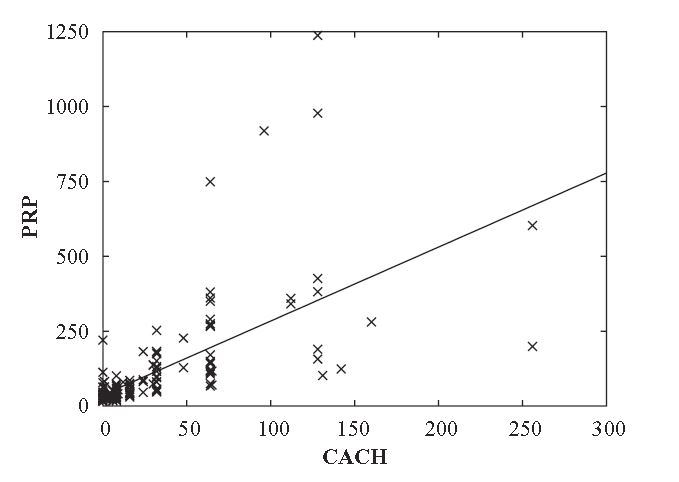
\includegraphics[width=3.0in]{linear-regression}
    \caption{Example of a line that fits a set of points according to linear regression; example taken from \cite{Witten} }
    \label{fig:linear-regression}
\end{figure}


\vspace{2mm}
Chen\cite{Chen} tries out a linear regression model for 120 parking spots and 1 hour ahead prediction. His $R^2$ value is 92\% and MAPE is close to 8\%.

\subsubsection{Support Vector Regression (SVR)}
Support Vector Regression is a prediction method applicable also for non-linear models. Compared to linear regression, it distinguishes itself by fitting future points using a non-linear combination of support vectors, i.e. selected points from the current set. During the training phase, the support vectors are selected as the points that fall outside the $\epsilon$ error value range (see Figure~\ref{fig:svr}). The error is measured in absolute value and only accounts for points outside the $2\epsilon$ range. 

$$x = b + \sum_{i\:support\:vector} \alpha_i (a(i) \cdot a)  $$
where $b$ and $\alpha_i$ are determined in the training phase, $a(i)$ are the support vectors and $a$ is the current instance.  The dot product term is called the kernel function and is responsible for non-linear behavior when it contains higher order factors. There are various kernel functions used and choosing a good one for one's case is not trivial. As a whole, the algorithm tends to both minimize the error and simultaneously to maximize the flatness of the regression function, thus avoiding overfitting, i.e. over-training the model. 

\begin{figure}[!ht]
    \centering
    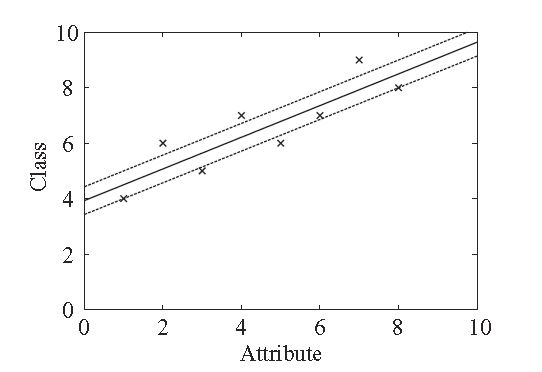
\includegraphics[width=3.0in]{svr}
    \caption{Example of a line determined by SVR; some points lie outside the $2\epsilon$-wide band; example taken from \cite{Witten} }
    \label{fig:svr}
\end{figure}

\vspace{2mm}
Chen\cite{Chen} constructs vectors of 24 elements that represent parking values corresponding to the last 24 hours and uses Support Vector Regression to predict future values:

$$y(t+1) = w^T\gamma(x_k(t)) + b$$
where $x_k(t)$ holds parking data $y(t-k+1), y(t-k+2), ..., y(t)$. The application of this model yields a MAPE value of about 7\% for about 100 parking spots.

\subsubsection{ARIMA}
In time series analysis autoregressive integrated moving average (ARIMA), models are used to forecast future points in the series. The autoregressive (AR) part accounts for its own lagged (i.e. previous) values, while its moving average (MA) part computes future values using past prediction errors. An ARIMA model predicts future values using its both components. Its prerequisite is that the data has to be stationary, i.e. its mean and variance are constant over time. In order to achieve that, the time series at hand may be differentiated (i.e. replace current point with the difference to its previous point) more times. $ARIMA(p,d,q)$ stands for a model that has been differentiated $d$ times, looks behind at its last $p$ values and at its previous $q$ prediction errors. An $ARIMA(p,d,q)(P,D,Q)_m$ is a seasonal model that recognizes some temporary behavior based on reoccurring events of period $m$.

\vspace{2mm}
Chen\cite{Chen} uses an $ARIMA(2,0,1) x (1,1,0)_{24}$ model with the seasonal factor corresponding to the hours of the day. He measures a MAPE error ratio for 100+ parking spots for 1 hour ahead of about 6\%.

\vspace{2mm}
Rajabioun and Ioannou\cite{Rajabioun} propose a multivariate autoregressive model that takes into account not only temporal but also spatial correlations of parking availability. They observe that the nearer the parking spots are, the more similar the occupancy rates are. Their model yields a 14\% MAPE for a 20-minute prediction horizon.

\subsubsection{Neural Networks}
Neural Networks (NN) relax the conditions of linearity and stationarity that the previous models impose and hence may achieve new levels of accuracy. They consists of a directed graph that contains nodes (i.e. neurons) with a  activation function, which map inputs to an output values. In particular, Multilayer Perceptrons (MLP) are models where the activation function is non-linear. Apart from the input and output layers, MLPs have one or more hidden layers. Learning occurs by changing the weights in the activation functions by observing the error between the output and expected result. This supervised learning method is called backpropagation.

\vspace{2mm}
Vlahogianni et al.\cite{Vlahogianni} use a MLP with 8 hidden layers for a 4\% MAPE 1 hour prediction error. Chen\cite{Chen} achieves a 3\% error when using 2-hidden layer NN for an 1 hour-ahead prediction.

\subsubsection{Continuous Markov Chains}
Markov Chains are used to model processes in which future states depend causally only on the current state and not on previous states. Between any two states there may be a transition probability which expresses how likely the process is to jump from one state to the other. Markov Chains can be either discrete- or continuous-time. For the latter the time spent in each state has an exponential distribution, i.e. states transitions at fixed time intervals.

\vspace{2mm}
In the case of parking, this model seems to apply. Future parking configurations indeed depend solely on the current configuration. Caliskan et al.\cite{Caliskan2007} defines a state of the process by the absolute occupancy value. The authors consider the average parking arrival rate and the average parking rate (i.e. inverse of parking duration) to construct a Continuous-Time Markov Chain (CTMC) and to predict future occupancy values. In Figure~\ref{fig:markov-chain}, the CTMC is represented by $\lambda$ (parking arrival rate) and $\mu$ (parking rate). The authors do not provide an exact error measure for their application of the model, however state that "our prediction algorithm is most effective for prediction times up to 15 minutes [..] with increasing prediction time, the uncertainty of the model increases".

\begin{figure}[!ht]
    \centering
    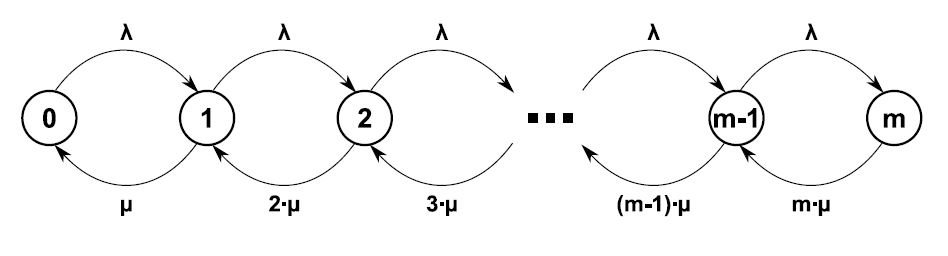
\includegraphics[width=4.0in]{markov-chain}
    \caption{Continuous-Time Markov Chain corresponding to a Parking Location; taken from \cite{Caliskan2007}}
    \label{fig:markov-chain}
\end{figure}

To summarize the presented methods, we outline their main features in Table~\ref{tab:methods}. An exact error-comparison based on the same testing ground is, at this point, not available. Individual testing results have been provided in their corresponding paragraphs.

%\bgroup
%\def\arraystretch{1.5}%  1 is the default, change whatever you need
{\footnotesize
\begin{table}[!ht]
 \centering
 {\renewcommand{\arraystretch}{2.5}
	\resizebox{\textwidth}{!}{
  \begin{tabular}{ | c | c | c | }
    \hline
     & \textbf{Recommending features} & \textbf{Limitations} \\ \hline
    \textbf{Linear Regression} & \begin{minipage}{0.4\textwidth} general and simple prediction method \end{minipage} & \begin{minipage}{0.4\textwidth} only matches linear models \end{minipage} \\ \hline
    \textbf{SVR} & \begin{minipage}{0.4\textwidth} additionally fits non-linear models \end{minipage} & \begin{minipage}{0.4\textwidth}choosing kernel function\end{minipage} \\ \hline
    \textbf{ARIMA} & \begin{minipage}{0.4\textwidth} applies directly to time-series \end{minipage} & \begin{minipage}{0.4\textwidth}requires linearity and stationarity \end{minipage} \\ \hline
	\textbf{Neural Networks} & \begin{minipage}{0.4\textwidth}adaptable to latest observed results via backpropagation \end{minipage} & \begin{minipage}{0.4\textwidth} proneness to overfitting; its "black box" nature \end{minipage} \\ \hline
	\textbf{Markov Chains} & \begin{minipage}{0.4\textwidth} models processes of independent events\end{minipage} & \begin{minipage}{0.4\textwidth}does not accommodate other features than time-related ones \end{minipage}\\ \hline
  \end{tabular}}}
	\caption{Prediction Method Summary}
 	\label{tab:methods}
\end{table}}
%\egroup

 
\section{Implementation}
The implementation will be done at SoNah UG. The software component will be realised in Java or Python. It remains to be decided whether it will take the form of a library or will integrate with the UI in an MVC application (e.g. in Django). Databases used will be a NoSQL (e.g. MongoDB) and a relational database (e.g. MySQL).

\subsection{Evaluation}
A fraction of the accumulated live parking data will be used towards training the model. We estimate to use  10-30\% of the data for testing, depending on how consolidated the model already is.

\vspace{2mm}
Test data can be alternatively simulated, in case not enough parking data was collected by that time.

\section{Research Goals}
\begin{enumerate}
\item How is the live parking data obtained and how is it stored/retrieved? What about historical data?
\item How is the parking data associated to geo-locations realised?
\item How much data is needed to start building a prediction model with? In what degree can "parking profiles" be extrapolated that fit areas with little or no data?
\item How accurate can a system predict availability of free parking spots and minimize walking distances given parking information data collected from sensors, parking meters and user-generated via smartphone application?
\end{enumerate}

\section{System components and architecture}
The Parking Information System is envisioned to have the following structure:
{\small
\begin{longtable}{| c | >{\raggedright\arraybackslash}p{9cm} |}%[!ht]
 %\centering
  %\begin{tabular}{ | c | >{\raggedright\arraybackslash}p{9cm} | }
    \hline
     & \multicolumn{1}{c|}{\textbf{Queries}} \\ \hline
    \textbf{Parking sensor} & \tabitem Observes that a parking spot becomes free \\ 
     		   & \tabitem Observes how many free parking spots for a parking location are free \\ \hline 
    \textbf{Analytics} & \tabitem Computes the probability that a parking location has at least one free spot in the future \\ \hline
    \textbf{User} & \tabitem Finds out what parking location has at least one spot free \\ 
    	& \tabitem Finds out how many free spots does a parking location have at a certain time of the day \\ \hline
  %\end{tabular}
	\caption{Functionality on different levels}
 	\label{tabelle}
\end{longtable}}

The Analytics component exchanges information with the other components (see Figure~\ref{fig:architektur}). The User-Interface queries Analytics on parking spot availability, and receives a synchronous answer. Incoming data from sensors and from other sources contributes to building the prediction model asynchronously.

\vspace{4mm}
\begin{figure}[!ht]
    \centering
    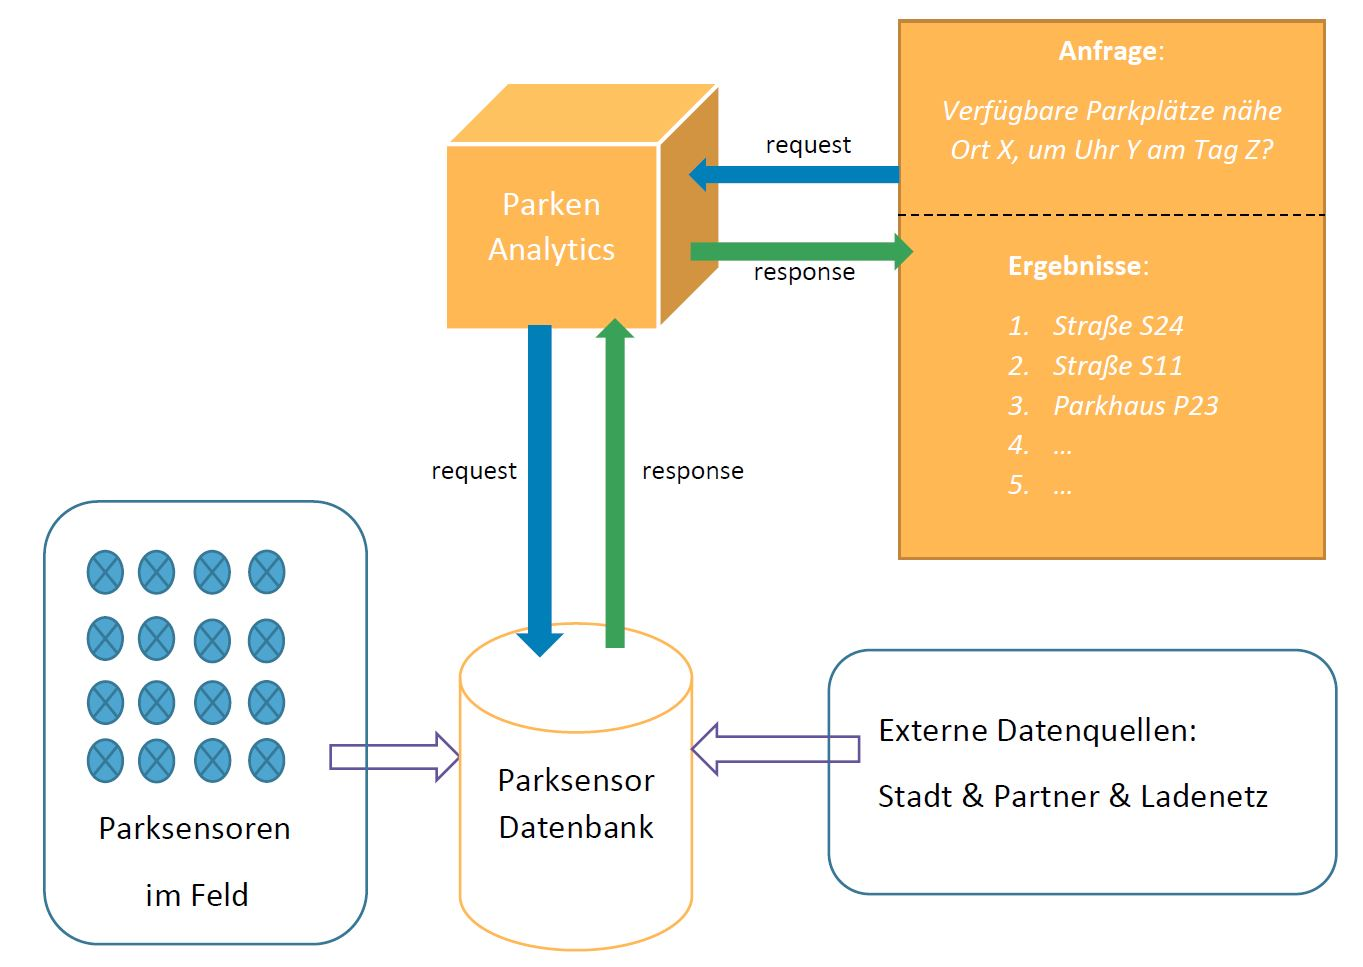
\includegraphics[width=4.5in]{Architektur}
    \caption{System components and their interaction}
    \label{fig:architektur}
\end{figure}

\section{Parking profiles}
Apart from answering queries for specific times, SoNah is envisioned to provide a graph with average parking
rates per parking location per day (see Figure~\ref{stosszeiten}).. Various factors like the day of the week, whether it is a holiday or an event is taking place play an important role.

\begin{figure}[!ht]
    \centering
    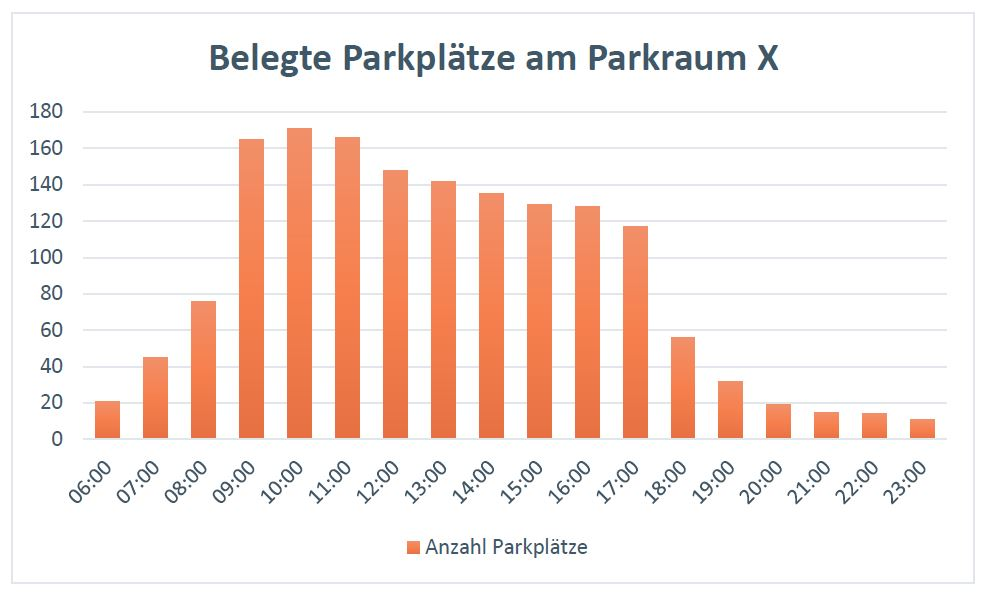
\includegraphics[width=4.0in]{Stosszeiten}
    \caption{Parking profile for a parking location}
    \label{stosszeiten}
\end{figure}

\section{Timeplan}

\nocite{*}

\printbibliography

\end{document}